\providecommand{\main}{..}
\documentclass[\main/main.tex]{subfiles}
\begin{document}

\chapter{Analisi teorica di prestazioni}
\begin{multicols}{2}
\begin{observation}[Di cosa si occupa l'analisi teorica di prestazioni?]
    L'analisi teorica di prestazioni si occupa di dimostrare che l'algoritmo fornisce soluzioni con una data garanzia di qualità, sempre o con una data frequenza.
\end{observation}
\begin{definition}[Differenza assoluta]
Chiamiamo la soluzione euristica \(f_A(l)\) e quella ottima \(f^*(l)\), allora la \textbf{differenza assoluta} è definita come:
  \[
    \tilde{\delta}_A(l) = \abs{f_A(l) - f^*(l)} \geq 0
  \]
  Dipende dall'unità di misura dell'obbiettivo e pertanto si usa di rado.
\end{definition}

\begin{definition}[Differenza relativa]
Chiamiamo la soluzione euristica \(f_A(l)\) e quella ottima \(f^*(l)\), allora la  \textbf{differenza relativa} è definita come:
  \[
    \delta_A(l) = \frac{\abs{f_A(l) - f^*(l)}}{f^*(l)} \geq 0
  \]
  È frequente nell'analisi sperimentale.
\end{definition}

\begin{definition}[Rapporto di approssimazione]
Chiamiamo la soluzione euristica \(f_A(l)\) e quella ottima \(f^*(l)\), allora il  \textbf{rapporto di approssimazione} è definito come:
  \[
    \rho_A(l) = \max \sqr{\frac{f_A(l)}{f^*(l)}, \frac{f^*(l)}{f_A(l)}} \geq 1
  \]
  È frequente nell'analisi teorica.
\end{definition}
\end{multicols}

\section{Analisi teorica nel caso pessimo}
\begin{multicols}{2}
\begin{definition}[Approssimazione assoluta]
Il fattore \(\bar{\alpha}_A\) si dice garanzia di approssimazione assoluta:
\[
    \exists \bar{\alpha}_{A} \in \N: \bar{\delta}_A(I) \leq \bar{\alpha}_A \quad \forall I \in \mathbb{I}
\]
Un esempio (raro) è l'algoritmo di Vizing per l'Edge Coloring \(\rnd{\bar{\alpha} = 1}\).
\end{definition}
\begin{definition}[Approssimazione relativa]
Il fattore \(\alpha_A\) si dice garanzia di approssimazione relativa:
\[
    \exists \alpha_A \in \R^+: \rho_A(I) \leq \alpha_A \quad \forall I \in \mathbb{I}
\]
\end{definition}
\begin{observation}[Garanzia e dimensione dell'istanza]
    In generale, la garanzia dipende dalla dimensione dell'istanza:
    \[
        \rho_A(I) \leq \alpha_A(n) \quad \forall I \in \mathbb{I}_n, n \in \N
    \]
    Contrariamente all'efficacia, per l'efficienza potrebbe anche non esserne dipendente.
\end{observation}
\begin{analysis}[Ricavare la garanzia di approssimazione]
    Per un problema di minimizzazione si vuole dimostrare che \(f_A(I) \leq \alpha f^*(I) \quad \forall I \in \mathbb{I}\).
\begin{enumerate}
    \item Si trova un modo per costruire una \textbf{stima per difetto} \(LB(I)\):
    \[
        LB(I) \leq f^*(I) \quad I \in \mathbb{I}
    \]
    \item Si trova un modo per costruire una stima per eccesso \(UB(I)\), che sia legata a \(LB(I)\) da un coefficiente \(\a\), o da una funzione \(\a\rnd{n}\):
    \[
        UB(I) = \alpha LB(I) \quad I \in \mathbb{I}
    \]
    \item Si trova un algoritmo \(A\) la cui soluzione non è peggiore di \(UB(I)\):
    \[
        f_A(I) \leq UB(I) \quad I \in \mathbb{I}
    \]
    \item Quindi \(f_A(I) \leq UB(I) = \alpha LB(I) \leq \alpha f^*(I) \quad \forall I \in \mathbb{I}\):
    \[
        f_A(I) \leq \alpha f^* (I) \quad \forall I \in \mathbb{I}
    \]
\end{enumerate}
\end{analysis}
\end{multicols}
\clearpage
\section{Algoritmo 2-approssimato per il VCP}
\begin{multicols}{2}
\begin{definition}[Algoritmo 2-approssimato per il VCP]
    Dato un grafo non orientato \(G = \rnd{V, E}\) si cerca il sottoinsieme di vertici di cardinalità minima tale che ogni lato del grafo vi incida.
\end{definition}
\begin{definition}[Matching]
Si dice \textbf{matching} un insieme di lati non adiacenti fra loro.
\end{definition}
\begin{definition}[Matching massimale]
Un matching viene detto massimale quando è tale che qualsiasi altro lato del grafo è adiacente a un lato del matching.
\end{definition}
\begin{definition}[Algoritmo del matching]
    \begin{enumerate}
        \item Si costruisce un matching massimale \(M \subseteq E\) cioè tale che ogni altro lato di \(E\) è adiacente a un lato di \(M\).
        \item L'insieme dei vertici estremi dei lati del matching è una soluzione, che può essere migliorata eliminando dei vertici ridondanti:
        \[
            x_A = \bigcup_{\rnd{u,v} \in M} \crl{u,v}
        \]
    \end{enumerate}
\end{definition}
\begin{proof}[L'algoritmo del matching è 2-approssimato]
    \begin{enumerate}
        \item La cardinalità del matching \(M\) è una stima per difetto \(LB(I)\).
        \begin{enumerate}
            \item La cardinalità di una copertura ottima per qualsiasi sottoinsieme di lati \(E' \subseteq E\) non supera quella di una copertura ottima per \(E\) (coprire tutti i lati costa di più che coprire solo i lati del matching):
            \[
                \abs{x^*_{E'}} \leq \abs{x^*_E}
            \]
            \item La copertura ottima di un matching \(M\) ha cardinalità \(\abs{M}\), cioè per ogni lato del matching basta e occorre un vertice diverso.
        \end{enumerate}
        \item Includendo entrambi i vertici di gni lato nel matching si ottiene una stima per eccesso che copre sia il matching, sia i lati adiacenti, che risulta di valore \(UB(I) = 2LB(I)\), cioè vi sono due vertici diversi per ogni lato.
        \item L'algoritmo del matching dà soluzioni di valore \(f_A(I) \leq UB(I)\) (scremando i vertici ridondanto se ve ne sono).
    \end{enumerate}
    
    Ne deriva che \(f_A(I) \leq 2f^*(I) \quad \forall I \in \mathbb{I}\) cioè \(\alpha_A = 2\).
\end{proof}
\begin{definition}[Schema di approssimazione]
Uno \textbf{Schema di Approssimazione} è un algoritmo \(A\) parametrico con \(\alpha\) a piacere:
\[
    T_{A_\alpha} \in O\rnd{f\rnd{n, \alpha}} \quad \alpha \in [1; + \infty)
\]

Uno schema di approssimazione può essere:
\begin{description}
\item[Polinomiale] se \(f\rnd{n,\a}\) è un polinomio in \(n \quad \forall \alpha\) fissato.
\item[Pienamente polinomiale] se \(f\rnd{n, \a}\) è un polinomio in \(n\) e in \(\frac{1}{\a}\)
\end{description}
\end{definition}
\begin{observation}[Esistenza di problemi non approssimabili]
    È importante tenere a mente che esistono \textbf{problemi non approssimabili}, cioè problemi per cui l'unico algoritmo approssimato è un algoritmo esatto: un esempio è il TSP, che contiene istanze non approssimabili.
\end{observation}
\begin{observation}[Quando è possibile approssimare il TSP?]
    In alcune istanze del TSP è lecito considerare:
    \begin{enumerate}
        \item Il grafo \(G = \rnd{N, A}\) completo.
        \item La funzione \(c\) sia una distanza valida: cioè goda di simmetria e disuguaglianza triangolare.
    \end{enumerate}
\end{observation}
\begin{definition}[Algoritmo del doppio albero]
\begin{enumerate}
    \item Consideriamo il grafo completo non orientato corrispondente a \(G\).
    \item Costruiamo un albero ricoprente di costo minimo \(T^* = \rnd{N, X^*}\).
    \item L'insieme \(x\) degli archi di \(G\) corrispondenti ai lati di \(X^*\) forma un ciclo orientato che passa per ogni nodo, in generale più volte.
    \item Finché ci sono nodi con più di un arco uscente ed entrante:
    \begin{enumerate}
        \item Si sceglie un nodo qualsiasi \(j\) e una coppia di archi \(\rnd{i,j}\) e \(\rnd{j,k}\) in \(x'\).
        \item Si sostituisce la coppia di archi con l'arco diretto.
        \[
            x = x \setminus \crl{\rnd{i,j}, \rnd{j, k}} \cup \crl{\rnd{i,k}}
        \]
    \end{enumerate}
\end{enumerate}
\end{definition}
\begin{proof}[L'algoritmo del doppio albero è 2-approssimato]
\begin{enumerate}
    \item Il costo dell'albero ricoprente minimo è una stima per difetto \(LB(I)\): togliendo un arco a un ciclo hamiltoniano si ottiene un cammino hamiltoniano meno costoso e un cammino hamiltoniano è un particolare tipo di albero ricoprente.
    \item Sostituendo ogni lato dell'albero con due archi opposti si ottiene una stima per eccesso, essendo un cammino hamiltoniano, di valore \(UB(I) = 2LB(I)\), cioè due archi sostituiscono ogni lato.
    \item L'algoritmo del doppio albero dà soluzioni di valore \(f_A(I) \leq UB(I)\), cioè sostituendo due archi consecutivi con uno diretto il costo cala.
\end{enumerate}

Ne deriva che \(f_A(I) \leq 2f^*(I) \forall I \in \mathbb{I}\), cioè \(\a_A = 2\).
\end{proof}
\begin{definition}[Algoritmo randomizzato approssimato]
L'algoritmo esegue operazioni che non dipendono solo dai dati, ma anche da numeri pseudocasuali: per un tale algoritmo \(A\) \(f_A(I)\) e \(\rho_A(I)\) sono variabili aleatorie.

Un \textbf{algoritmo randomizzato approssimato} ha un rapporto di approssimazione il cui valore atteso è limitato da una costante:
\[
    \mean{\rho_A(I)} \leq \a_A \quad \forall I \in \mathbb{I}
\]
\end{definition}

\begin{example}[Approssimazione randomizzata per Max-SAT]
Utilizzando un approccio puramente casuale, che assegna il valore di verità con probabilità \(\frac{1}{2}\), procediamo a determinare il valore atteso della soluzione:

Sia \(C_x \subseteq \crl{1, \ldots, m}\) l'insieme delle formule soddisfatte dalla soluzione \(x\).

Il valore dell'obbiettivo \(f(x)\) è il peso totale delle formule in \(C_x\), mentre il valore atteso rispetto a tutte le soluzioni \(x\) proposte dall'algoritmo \(A\) é:
\[
    \mean{f_A(I)} = \mean{\sum_{i \in C_x} w_i} = \sum_{i \in C} \rnd{w_i \cdot \prob{i \in C_x}}
\]

Sia \(k_i\) il numero di letterali della formula \(i \in C\) e \(k_{min} = \min_{i \in C} k_i\):
\[
    \prob{i \in C_x} = 1 - \rnd{\frac{1}{2}}^{k_i} \geq 1 - \rnd{\frac{1}{2}}^{k_{min}} \quad \forall i \in C
\]
Ne segue che:
\[
    \mean{f_A(I)} \geq \sum_{i \in C} w_i \cdot \sqr{1 - \rnd{\frac{1}{2}}^{k_{min}}} = \sqr{1 - \rnd{\frac{1}{2}}^{k_{min}}} \sum_{i \in C} w_i
\]
E siccome:
\[
    f^*(I) \leq \sum_{i \in C} w_i \quad \forall I \in \mathbb{I} \quad \text{e} \mean{\rho_A(I)} = \frac{f^*(I)}{\mean{f_A(I)}}
\]
Si ottiene:
\[
    \mean{\rho_{A}(I)} \leq \frac{1}{\sqr{1 - \rnd{\frac{1}{2}}^{k_{min}}}} \leq 2
\]
\end{example}
\end{multicols}
\chapter{Analisi sperimentale}
\begin{multicols}{2}
\begin{observation}[Di cosa si occupa l'analisi sperimentale?]
L'analisi sperimentale indaga le leggi che regolano il comportamento degli algoritmi:

Si tratta di:
\begin{enumerate}
    \item Ottenere indici di efficacia e di efficienza di un algoritmo.
    \item Descrivere il legame fra gli indici di efficacia o efficienza e valori parametrici delle istanze.
    \item Confrontare l'efficacia di algoritmi diversi per indicare il migliore.
    \item Suggerire miglioramenti all'algoritmo.
\end{enumerate}
\end{observation}
\begin{definition}[Campione significativo]
    Non potendo testare tutte le istanze, occorre definire un campione. Un campione significativo deve rappresentare:
    \begin{description}
        \item[Diverse dimensioni] cosa particolarmente importante per l'analisi sperimentale della complessità.
        \item[Caratteristiche strutturali] come è "fatto" il modello dei dati.
        \item[Tipologie di applicazione] logistica, telecomunicazioni, produzione...
        \item[Tipologie di generazione] realistiche, artificiali, trasformazioni di altri problemi...
        \item[Tipologie di distribuzione probabilistica] uniforme, normale, esponenziale...
    \end{description}
    Tipicamente si cerca di concentrarsi sulle istanze \textbf{più frequenti in pratica}, in particolare quelle \textbf{più difficili} ma evitando quelle che \textbf{richiedono troppo tempo}.
\end{definition}
\begin{definition}[Benchmark]
     Un Benchmark considera l'esecuzione di un algoritmo \(A\) come un esperimento casuale: un'analisi significativa è possibile solo tenendo fissa la dimensione \(n\) (con gli altri parametri rilevanti suggeriti dall'analisi del caso pessimo).
\end{definition}
\begin{observation}[Cosa costituisce lo spazio degli esiti di un Benchmark?]
    Lo \textbf{spazio degli esiti} è costituito dall'insieme delle istanze \(\mathcal{I}_n\).
\end{observation}
\begin{observation}[Quale è la variabile aleatoria sotto indagine di un Benchmark?]
    Il tempo di calcolo \(T_A(I)\) è la variabile aleatoria sotto indagine.
\end{observation}
\begin{observation}[Da cosa vengono descritte le prestazioni dell'algoritmo secondo il Benchmark?]
    Le prestazioni \(A\) sono descritte dalle proprietà statistiche di \(T_A(I)\), cioè il suo valore atteso e varianza in \(\mathcal{I}_n\).
\end{observation}
\begin{observation}[Cosa succede quando vengono fissati tutti i parametri rilevanti?]
    Per gli algoritmi polinomiali, se i parametri rilevanti sono fissati, la media tende ad essere un indice affidabile.
\end{observation}
\end{multicols}
\clearpage
\begin{multicols}{2}
\begin{definition}[Diagramma RTD]
    La funzione di distribuzione della variabile aleatoria \(T_A(I)\) in \(\mathcal{I}_n\) fornisce il diagramma della \textbf{Run Time Distribution (RTD)}.

    \begin{figure}
        \centering
        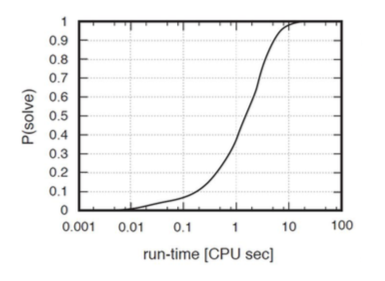
\includegraphics[width=\textwidth]{images/RTD.png}
    \end{figure}
    
    Quando tutti i parametri influenti sono stati individuati il diagramma \textbf{RTD} degenera in un gradino, vale a dire che il tempo è quasi uguale per tutte le istanze di \(\mathcal{I}_n\).
    
    Se è molto distribuito potrebbero esistere altri parametri interessanti.
\end{definition}
\begin{definition}[Diagramma di Scaling]
    La complessità asintotica indica per il caso pessimo una fascia di andamenti di ampiezza imprecisata.
    
    \begin{figure}
        \centering
        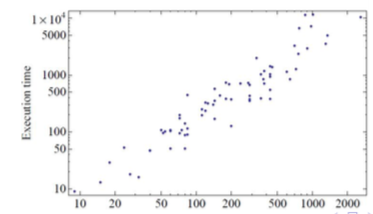
\includegraphics[width=\textwidth]{images/scaling.png}
    \end{figure}
    
    Lo studio empirico al variare di \(n\) fornisce quindi le informazioni mancanti.
    
    Per eseguirlo, bisogna:
    \begin{enumerate}
        \item Estrarre una sequenza di campioni \(\mathcal{I}_n\) per valori crescenti di \(n\).
        \item Applicare l'algoritmo e registrare i tempi \(T_A(I)\)
        \item Tracciare la nuvola dei punti \(\rnd{n, T(I)}\) o delle medie \(\rnd{n, \frac{\sum_{I\in \mathcal{I}_n} T(I)}{\abs{\mathcal{I}_n}}}\)
        \item Ipotizzare una famiglia di interpolanti con l'aiuto dell'analisi teorica
        \item Tarare i parametri dell'interpolante.
    \end{enumerate}
\end{definition}
\begin{observation}[Come si identifica la funzione interpolante?]
    Per identificare la funzione interpolante si procede per tentativi per capire su quale tipo di scala si genera un diagramma di scaling lineare.
\end{observation}
\begin{definition}[Funzione interpolante lineare]
    La funzione interpolante è lineare quando la scala risulta lineare sia su ascisse che su ordinate ed è definita come:
    \[
        T(n) = \a n + \beta \Leftrightarrow c_1 n + c_2 
    \]
\end{definition}
\begin{definition}[Funzione interpolante polinomiale]
    La funzione interpolante è polinomiale quando la scala risulta logaritmica sia su ascisse che su ordinate ed è definita come:
    \[
        \log T(n) = \a \log n + \beta \Leftrightarrow 2^\beta n^\alpha
    \]
\end{definition}
\begin{definition}[Funzione interpolante esponenziale]
     La funzione interpolante è esponenziale quando la scala risulta semi-logaritmica, cioè lineare su ascisse e logaritmica sulle ordinate ed è definita come:
     \[
        \log T(n) = \alpha n + \beta \Leftrightarrow 2^\beta \rnd{2^\alpha}^n
    \]
\end{definition}
\end{multicols}
\section{Analisi dell'efficacia di un algoritmo}
\begin{multicols}{2}
\begin{observation}[Come procede l'analisi dell'efficacia di un algoritmo]
    Considerando l'esecuzione di un algoritmo \(A\) come un esperimento casuale: 
\begin{enumerate}
    \item L'insieme delle istanze \(\mathcal{I}_n\) costituisce lo \textbf{spazio degli esiti}.
    \item La differenza relativa \(\delta_A(I)\) è la variabile aleatoria sotto indagine.
\end{enumerate}
Le prestazioni di \(A\) sono descritte dalle proprietà statistiche di \(\delta_A(I)\).
\end{observation}
\begin{definition}[Solution Quality Distribution (SQD)]
Una descrizione completa di \(\delta_A(I)\) è data dalla funzione di distribuzione:
\[
    F_A\rnd{\alpha} = \prob{\delta_A(I) \leq \alpha} \quad \forall \a \in \R
\]
Il suo andamento è il diagramma SQD.

Per un qualsiasi algoritmo, la funzione di distribuzione di \(\delta_A(I)\) è \textbf{monotona non decrescente}, \textbf{nulla per \(\alpha < 0\)} e tenda a \(1\) per \(\alpha \rightarrow + \infty\).

In particolare:
\begin{description}
    \item[Per algoritmi esatti] è una funzione a gradino, pari a \(1 \quad \forall \alpha \geq 0\)
    \item[Per algoritmi \(\bar{\a}\)-approssimati] è una funzione pari a \(1 \quad \forall \alpha \geq \bar{\alpha}\)
\end{description}
\end{definition}
\begin{observation}[Come generare il diagramma SQD]
    Per generare il diagramma SQD in pratica si ricostruisce un \textbf{diagramma campionario} della funzione:
    \begin{enumerate}
        \item Si genera un campione \(\bar{\mathcal{I}} \subset \mathcal{I}\) abbastanza grande di istanze indipendenti.
        \item Si applica l'algoritmo a ogni istanza \(I \in \bar{\mathcal{I}}\) e si costruisce l'insieme:
        \[
            \Delta_A\rnd{\bar{\mathcal{I}}} = \crl{\delta_A(I): I \in \bar{\mathcal{I}}}
        \]
        \item Si ordina per valori non decrescenti.
        \item SI riportano nel grafico i punti \(\rnd{\delta_j, \frac{j}{\abs{\bar{\mathcal{I}}}}} \quad \forall j \in 1, \ldots, \abs{\bar{\mathcal{I}}}\)
    \end{enumerate}
    Spesso vengono realizzati numerosi diagrammi al variare di qualche parametro di interesse per l'algoritmo.
\end{observation}
\end{multicols}
\clearpage
\subsection{Test di Wilcoxon}
\begin{definition}[Test di Wilcoxon]
    Il \textbf{test di Wilcoxon} valuta la differenza fra i risultati dei due algoritmi \(\delta_{A_1}(I) - \delta_{A_2}(I)\):
\begin{enumerate}
    \item Si formula l'ipotesi nulla \(H_0\): la differenza ha mediana nulla.
    \item Si estrae un campione di istanze \(\bar{\mathcal{I}}\) e gli si applicano i due algoritmi, ottenendo un campione di coppie di valori \(\rnd{\delta_{A_1}, \delta_{A_2}}\).
    \item Si calcola la probabilità \(p\) di ottenere il risultato osservato o uno più estremo, supponendo vera l'ipotesi \(H_0\).
    \item Si sceglie un livello di significatività \(\bar{p}\), tipicamente \(5\%\) o \(1\%\), pari alla probabilità massima accettabile di rifiutare \(H_0\) qualora fosse vera.
    \item Se \(p \leq \bar{p}\) si rifiuta \(H_0\).
\end{enumerate}
\end{definition}
\begin{observation}[Quali ipotesi fa il test di Wilcoxon?]
Il test non fa ipotesi sulla distribuzione di probabilità dei valori testati, quindi è un test non parametrico e ciò lo rende adatto a valutare le prestazioni di algoritmi euristici, dato che la distribuzione della differenza relativa non è nota.

Fa però 3 ipotesi:
\begin{enumerate}
    \item I dati sono coppie di valori riferiti alla stessa popolazione.
    \item Ogni coppia di dati è estratta indipendentemente dalle altre.
    \item I dati sono misurate su scale almeno ordinali.
\end{enumerate}
\end{observation}
\begin{observation}[Esecuzione del test]
    \begin{enumerate}
        \item Calcola le differenze assolute \(\abs{\delta_{A_1}(I_i) - \delta_{A_2}(I_i)} \quad \forall i \in 1, \ldots, \abs{\bar{\mathcal{I}}}\).
        \item Le ordina per valori crescenti e attribuisce un rango \(R_i\) a ciascuna.
        \item Somma separatamente i ranghi delle coppie con differenza positiva e quelli delle coppie con differenza negativa.
        \[
            \begin{cases}
                W^+ = \sum_{i: \delta_{A_1}(I_i)>\delta_{A_2}(I_i)} R_i\\
                W^- = \sum_{i: \delta_{A_1}(I_i)<\delta_{A_2}(I_i)} R_i\\
            \end{cases}
        \]
        Se l'ipotesi nulla \(H_0\) fosse vera, le due somme dovrebbero coincidere.
        \item La differenza fra \(W^+\) e \(W^-\) consente di calcolare il valore di \(p\): dati i \(2^{\abs{\bar{\mathcal{I}}}}\) esiti, corrispondenti a \(\abs{\bar{\mathcal{I}}}\) differenze positive o negative, si contano quelli con \(\abs{W^+ - W^-}\) pari o superiori all'osservazione.
        \item Se \(p < \bar{p}\), la differenza è significativa e un algoritmo prevale sull'altro:
        \begin{description}
            \item[Caso \(W^+ < W^-\):] significa che \(A_1\) è migliore di \(A_2\).
            \item[Caso \(W^+ > W^-\):] significa che \(A_1\) è peggiore di \(A_2\).
        \end{description}
    \end{enumerate}
\end{observation}
\begin{observation}[Che risultati può dare il test di Wilcoxon?]
    Il test di Wilcoxon può suggerire o che uno dei due algoritmi sia significativamente migliore dell'altro o che i due algoritmi sono statisticamente equivalenti.
    
    Se il campione è composto da classi di istanze parametricamente distinte, algoritmi complessivamente equivalenti potrebbero non esserlo sulle singole istanze.
    
    È sempre bene tenere a mente però che un algoritmo è migliore di un altro quando contemporaneamente ottiene risultati migliori e richiede un tempo inferiore.
\end{observation}
\clearpage
\section{Classificazione in base a tempo e qualità}
\begin{multicols}{2}
    \begin{definition}[Algoritmi completi o esatti]
        Gli algoritmi completi o esatti per ogni istanza \(I \in \mathcal{I}\) trovano l'ottimo in tempo finito.
    \end{definition}
    \begin{definition}[Algoritmi probabilisticamente approssimativamente completi]
        Gli algoritmi probabilisticamente approssimativamente completi per ogni istanza \(I \in \mathcal{I}\) la probabilità che trovino l'ottimo tende a \(1\) per \(t \rightarrow + \infty\).
    \end{definition}
    \begin{definition}[Algoritmi essenzialmente incompleti]
        Gli algoritmi essenzialmente incompleti sono algoritmi per cui esistono istanze per cui la probabilità di trovare l'ottimo rimane sempre \(<1\) per \(t\rightarrow + \infty\). Ne sono un esempio gli algoritmi greedy.
    \end{definition}
    \begin{observation}[Generalizzazione a soluzioni approssimate]
        Per generalizzare a soluzioni approssimate, si sostituisce la ricerca dell'ottimo con quella di un livello arbitrario \(\alpha\) di approssimazione.
    \end{observation}
    \begin{definition}[Algoritmi \(\alpha\)-completi]
        Gli algoritmi \(\alpha\)-completi sono algoritmi che per ogni istanza \(I \in \mathcal{I}\) trovano una soluzione \(\alpha\)-approssimata in tempo finito.
    \end{definition}
    \begin{definition}[Algoritmi probabilisticamente approssimativamente \(\alpha\)-completi]
        Gli algoritmi probabilisticamente approssimativamente \(\alpha\)-completi sono algoritmi che per ogni istanza \(I \in \mathcal{I}\) la probabilità che trovino una soluzione \(\alpha\)-approssimata tende a \(1\) per \(t \rightarrow + \infty\).
    \end{definition}
    \begin{definition}[Algoritmi essenzialmente \(\alpha\)-incompleti]
        Gli algoritmi essenzialmente \(\alpha\)-incompleti sono algoritmi che per cui esistono istanze per cui la probabilità di trovare una soluzione \(\alpha\)-approssimata rimane sempre \(<1\) per \(t\rightarrow + \infty\). 
    \end{definition}
\end{multicols}
\clearpage
\section{Probabilità di successo, diagrammi QRTD, SQD e SQT}
\begin{definition}[Probabilità di successo]
    Definiamo probabilità di successo \(\pi_{A, n}\rnd{\alpha, t}\) la probabilità che l'algoritmo \(A\) trovi in tempo \(\leq t\) una soluzione di livello \(\leq \alpha\):
    \[
        \pi_{A, n}\rnd{\alpha, t} = \prob{\delta_A(I, t) \leq \alpha |{I \in \mathcal{I}_n}}
    \]
    \begin{figure}
        \centering
        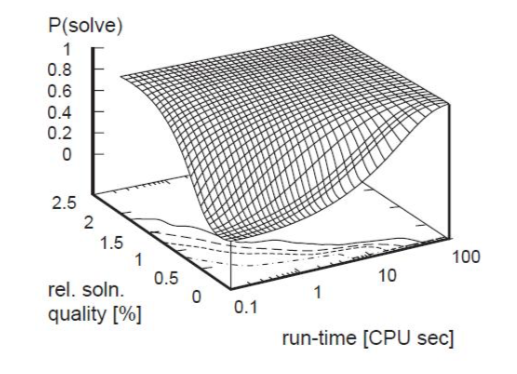
\includegraphics[width=0.5\textwidth]{images/probability.png}
    \end{figure}
\end{definition}
\begin{definition}[Diagrammi Qualified Run Time Distribution (QRTD)]
    I diagrammi QRTD descrivono l'andamento del tempo necessario a raggiungere dei prefissati livelli di qualità e sono utili quando il tempo di calcolo non è una risorsa stringente.
    \begin{figure}
        \centering
        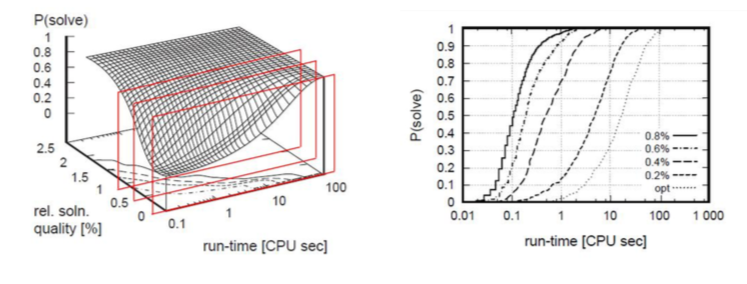
\includegraphics[width=\textwidth]{images/QRTD.png}
    \end{figure}
\end{definition}
\begin{definition}[Diagrammi Solution Quality Distribution (SQD)]
    I diagrammi SQD descrivono l'andamento del livello di qualità raggiunto in un dato tempo di calcolo e sono utili quando il tempo do calcolo è una risorsa stringente.
    \begin{figure}
        \centering
        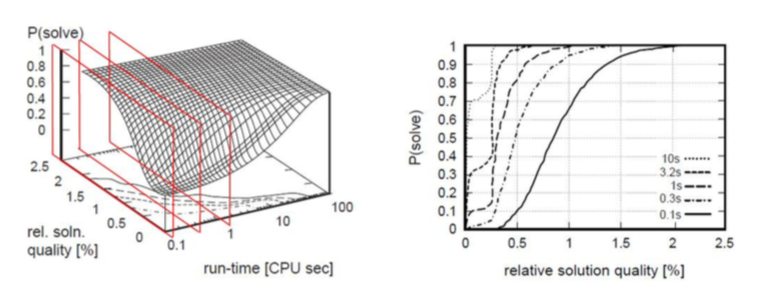
\includegraphics[width=\textwidth]{images/SQD.png}
    \end{figure}
\end{definition}
\begin{definition}[Diagrammi Solution Quality statistics over Time (SQT)]
    Sono diagrammi rappresentanti le linee di livello associate ai diversi quantili, che descrivono un compromesso fra qualità e tempo di calcolo. Un algoritmo robusto avrà linee molto ravvicinate tra loro.
    \begin{figure}
        \centering
        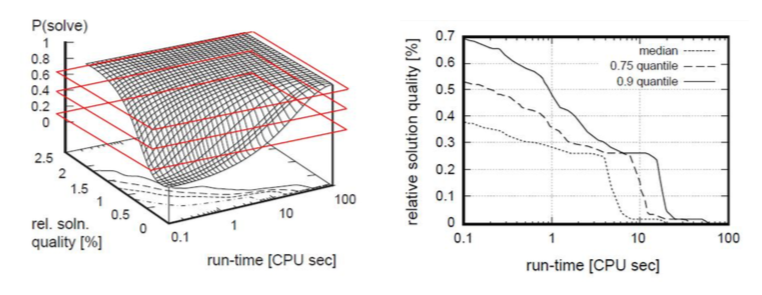
\includegraphics[width=\textwidth]{images/SQT.png}
    \end{figure}
\end{definition}
\end{document}